

% trial .tex file %
\documentclass[9pt]{article}  % specifies document class (article) and point size (10pt)
\usepackage{graphicx}
\usepackage{polski}
\usepackage[utf8]{inputenc}
\usepackage{sidecap}
\usepackage{wrapfig}
\usepackage{subfig}
\usepackage{amsmath}
\usepackage{float}
\usepackage{enumerate}
\usepackage{listings}
\usepackage{listings}
\usepackage{color}

\definecolor{dkgreen}{rgb}{0,0.6,0}
\definecolor{gray}{rgb}{0.5,0.5,0.5}
\definecolor{mauve}{rgb}{0.58,0,0.82}

\lstset{frame=tb,
  language=R,
  aboveskip=3mm,
  belowskip=3mm,
  showstringspaces=false,
  columns=flexible,
  basicstyle={\small\ttfamily},
  numbers=none,
  numberstyle=\tiny\color{gray},
  keywordstyle=\color{blue},
  commentstyle=\color{dkgreen},
  stringstyle=\color{mauve},
  breaklines=true,
  breakatwhitespace=true,
  tabsize=3
}


\begin{document}               % starts document
\author{Michał Kubica}
\title{Modele Liniowe \\ Raport nr 3}       
\maketitle                     % constructs big, fancy title

\section{Zadanie 6}            % makes a section header




  \subsection{Znajdź moc odrzucenia hipotezy zerowej $\beta_1=0$}
  
  Na podstawie wzorów podanych na wykładzie obliczono moc testu, czyli prawdopodobieństwo odrzucenia hipotezy zerowej, gdy jest ona fałszywa.
  
  $0.8032105 \approx 80\% $

  Moc testu na poziomie 80\% jest konwencjonalnym poziomem mocy, który zazwyczaj się przyjmuje w badaniach i czasopismach naukowych.

  Kod w R

    \begin{lstlisting}
n=40
sig2=120 
ssx=1000
alpha=0.05

sig2b1=sig2/ssx;
tc=qt(1-alpha/2, n-2)
beta1=1
delta=beta1/sqrt(sig2b1)
1-pt(tc,n-2,delta)+pt(-tc,n-2,delta)
    \end{lstlisting}  

  \subsection{Wykres mocy od $\beta_1$}

  Następnie wyliczono moc testu względem $\beta_1$ i wykres przedstawiono poniżej.

    \begin{lstlisting}
beta1=seq(-2, 2, 0.01)
delta=beta1/sqrt(sig2b1)
moc=1-pt(tc,n-2,delta)+pt(-tc,n-2,delta)
plot(beta1,moc, main="Moc testu", type='l')
    \end{lstlisting}  
    
    Jeśli moc testu jest zbyt niska to zwiększa się prawdopodobieństwo popełnienia błędu drugiego rodzaju, czyli przyjęcia hipotezy zerowej, gdy jest ona fałszywa. Jest to istotne z tego względu, że może to prowadzić do tego, że wyniki istotne będą odrzucane, a jest to efekt niepożądany.



    \begin{figure}[H]
      \centering
      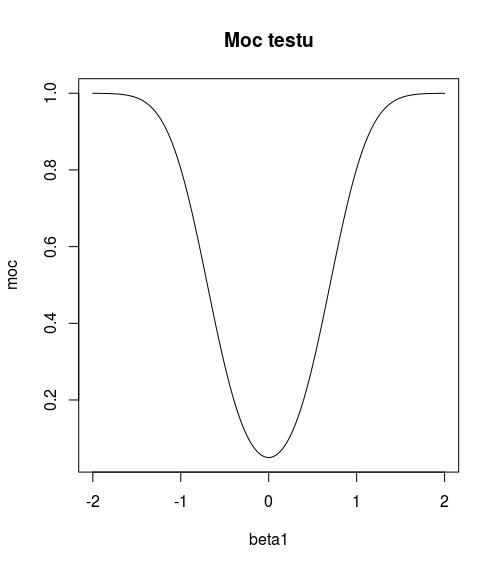
\includegraphics[width=1\textwidth]{6.png}
      \caption {Zależność mocy testu od beta1}
    \end{figure} 

    
\section{Zadanie 7}

Napisano funkcję, która przybliża prawdopodobieństwo odrzucenia hipotezy zerowej $\beta_1 = 0$ na podstawie wielokrotnej replikacji eksperymentu i wielokrotnego testowania hipotezy.   

a) 0.045

b) 0.049

c) 0.046

d) 0.057

Otrzymane wyniki są zbliżone do ustalonego poziomu istotności (prawdopodobieństwa odrzucenia hipotezy zerowej), co świadczy o poprawności wykonywanych replikacji.

    \begin{lstlisting}
f<-function(dim, n, beta1, dist)
{
  X = rnorm(dim, 0, 1/dim)
  if( dist == 1) {
    model = matrix(rnorm(dim*n, 0, 1), dim, n)
    } else 
    {
      model = matrix(rexp(dim*n, 1), dim, n)
    }
  model=apply(model, 2, function(eps){beta1*X+5+eps})
  model=apply(model, 2, function(Y){(summary(lm(Y~X))$coefficients[2,4] < alfa)})
  
  return(sum(model)/n)
}

f(200, 1000, 0, 1)
f(200, 1000, 0, 2)
f(200, 1000, 1.5, 1)
f(200, 1000, 1.5, 2)
    \end{lstlisting}  



\section{Zadanie 8}


  Mamy dane $n = 20$ obserwacji. Przetestowano model liniowy
  $Y = \beta_0 + \beta_1X + \epsilon$ używając estymatorów
  $b_0 = 1, b_1 = 3, s = 4$.


  \subsection{95\% przedział ufności dla $\beta_1$}
  Mając dane $s(b_1) = 1$ Wiemy, że przedział ufności dla $b_1 $ jest dany \newline
  $b_1 \pm t_c s(b_1)$, gdzie $t_c = (1-\alpha/2, n-2)$ \newline
  Dla $\alpha = 0.05$ i 18 stopni swodoby $t_c = 2.100922$ \newline
  Więc otrzymujemy przedział ufności \newline
  $3 \pm 2.100922$
  
  
  
  \subsection{Czy mamy pewność, że między X a Y jest zależność liniowa?}
  
    Pewności takiej nigdy nie możemy mieć. Ale ze względu na to, że 0 nie należy do wyliczonego przedziału ufności, możemy powiedzieć, że statystycznie mamy 95\% pewności, że ta zależność istnieje.
  
  \subsection{Prognoza dla $E(Y)$ kiedy $X =5$}

  95\% przedział ufności dla $E(Y)$ kiedy $X =5$

  Wprowadźmy oznaczenie,

    $$ A= \left[  \frac{1}{n} + \frac{(X_h-\bar{X})^2 }{\sum{(X_i-\bar{X})^2} }   \right] $$
    
    Wtedy
    
    $$ \hat{\mu}_H = 1+3 \cdot 5 = 16 $$
    
    $$t_c = s(\hat{\mu}_H) = 3$$
    
    $$ s^2(\hat{\mu}_H) = \frac{9}{{t_c}^2} = s^2 \cdot A$$
    
    $$A = \frac{9}{{t_c}^2 s^2}$$
    
    $$s^2(pred) = s^2(1+A) = s^2 \left(1+ \frac{9}{{t_c}^2 s^2} \right)$$
    
    $$t_c s(pred) = s \sqrt{{t_c}^2 +  \frac{9}{s^2}}  \approx 6.527 $$
    
    $$ 16\pm 6.527  = (9.473, 22.527)$$
    
    Wynik zgadza się z intuicją, ponieważ przedziały ufności są węższe.


    


    
    




\end{document}  







